\subsection{Транзакции. Восстановление. Алгоритм ARIES}

Про транзакции и восстановление БД после сбоев, можно прочитать в билете~\ref{tx-basics}.

\subsubsection{Алгоритм восстановления ARIES}

\paragraph{Фазы алгоритма}

\begin{itemize}
	\item \textbf{Разметка транзакций}. Каждая транзакция отмечается как
	      \textit{Redo} или \textit{Undo}.
	\item \textbf{Повторение истории}. Восстановление состояния системы на момент сбоя.
	\item \textbf{Откат транзакций}. Восстановление корректного состояния системы.
\end{itemize}

\paragraph{Фаза разметки транзакций}

Полностью эквивалентна классическому алгоритму. Может быть совмещена со следующей фазой.

\paragraph{Фаза повторения истории}

\begin{itemize}
	\item Чтение журнала идет от последней точки восстановления до конца.
	\item При чтении изменения оно применяется.
\end{itemize}

\paragraph{Фаза отката транзакций}

\begin{itemize}
	\item Чтение журнала идет по транзакциям из \textit{Undo}, от конца к началу.
	\item При чтении изменения оно откатывается.
\end{itemize}

\paragraph{Компенсационные записи}

В текущей версии алгоритма нет прогресса восстановления при повторном сбое. Добиться этого можно
путем введения \textbf{компенсационных записей}.

Будем производить следующие действия при необходимости отката изменений:

\begin{itemize}
	\item \textbf{Откат изменения};
	\item \textbf{Запись на диск};
	\item \textbf{Внесение компенсационной записи}. Запись означает, что откатываемое изменение, а
	      также все изменения, которые идут в логе позднее, были успешно откачены.
\end{itemize}

\begin{figure}[h]
	\centering
	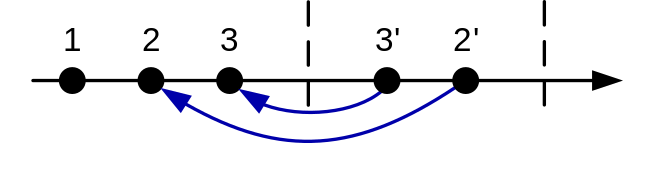
\includegraphics[width=0.8\textwidth]{../assets/kgeorgiy/transactions/Recovery_ARIES.svg.png}
	\caption{Иллюстрация компенсирующих записей при повторных сбоях}
	\label{recovery-aries}
\end{figure}

\begin{proposition}
	Компенсационные записи фиксируют прогресс восстановления БД и исключают повторный откат изменения
	при очередном восстановлении. Таким образом, повторные сбои не мешают завершению восстановления.
\end{proposition}

\subsubsection{Сравнение алгоритмов}

\paragraph{Число проходов}

\begin{itemize}
	\item \textbf{Классический алгоритм}. 3
	\item \textbf{Алгоритм ARIES}. 2
\end{itemize}

\paragraph{Рост журнала транзакций}

\begin{itemize}
	\item \textbf{Классический алгоритм}. В журнал добавляются записи отмены.
	\item \textbf{Алгоритм ARIES}. В журнал добавляются компенсирующие записи.
\end{itemize}

\paragraph{Повторные сбои}

\begin{itemize}
	\item \textbf{Классический алгоритм}. Полный перезапуск процесса восстановления.
	\item \textbf{Алгоритм ARIES}. Постепенное завершение.
\end{itemize}
